\documentclass{article}
\usepackage[normalem]{ulem}
\usepackage[utf8]{inputenc}
\usepackage{graphicx}
\usepackage{mathtools}
\usepackage{amssymb}
\usepackage{amsmath}
\usepackage{macros}
\usepackage{color}

\begin{document}

\section{Koder}
\subsection{Intro}
Rätta till mottagna meddelanden

NASA ville skicka en sond till mars. Skicka data väldigt långt. En tredjedel av bilden var fel.
Man kan inte skicka samma bild 8 ggr. Man vill ha små signaler.

\section{Kodning}
$x$ binär sträng.
$$x = 01100 = x_1 x_2 x_3 x_4 x_5 = ( x_1,x_2,\cdots, x_5 ) $$
$C=\{$kodord$\}$ = binära tal av samma längd

\subsection{Binär addition}
$$ 0+0=0 $$
$$ 0+1=1+0=1 $$
$$ 1+1=0 $$

\subsection{Summa av kodord}
$$ 0110+1010=(0 1 1 0)^T+(1 0 1 0)^T=(1 1 0 0)^T=1100 $$
Obs $x-y = x+y$, $x+x=0$

\subsection{Exempel}
$$ C=\{0,1\} $$
$$ x\to 1 $$

\subsection{Exempel}
$$ C=\{00,11\} $$
$$ x\to 10 $$
Fel! Vi kan ej veta om $x$ skulle vara 1 eller 0.

\subsection{Exempel}
$$ C=\{000,111\} $$
$$ x\to 001 $$ Rättat felet.
Det är större sannolikhet att $x$ är 0.
Närmsta granne rätt.

\subsection{Exempel}
$$ C=\{00,10,01,11\} $$
$$ x\to 10 $$
Vi kan ej veta vilket det menade meddelandet var om något gick fel.

\subsection{Definition}
Hamming\uline{avståndet} mellan två kodord $x$ och $y$ är
$d(x,y)=$ antalet positioner där $x$ och $y$ är olika.
Kodens separation (minsta avstånd).
$$d(C)=\min \{d(x,y);x,y\in C\}$$

\subsection{Exempel}
$$ C=\{010101, 101010, 111000, 000111\} $$
$$ d(101010, 000111) = 4$$
$$ d(C) = d(101010, 111000) = 2$$

\subsection{Sats}
Om $d(C)=k$ kan alla fel som påverkar $k-1$ bitar upptäckas\\
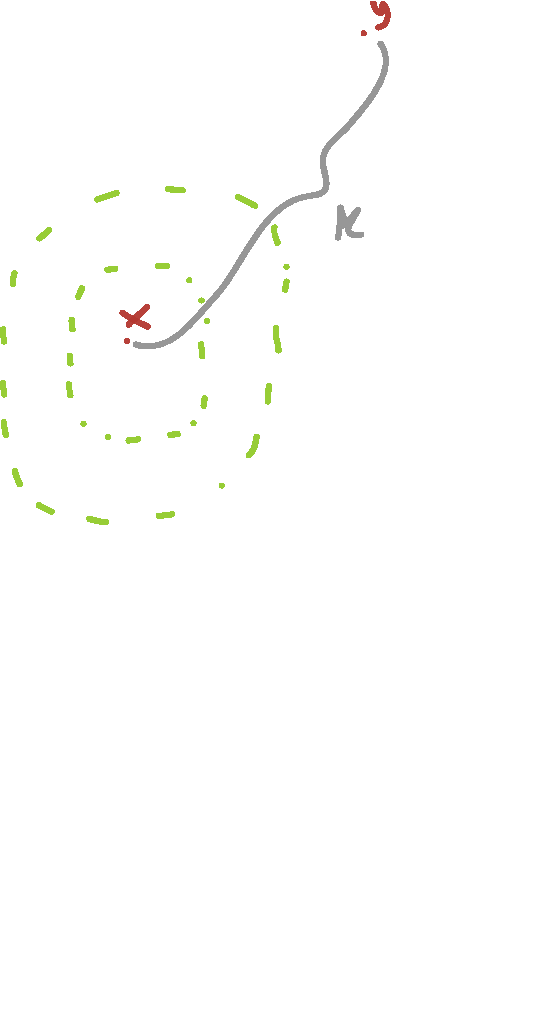
\includegraphics[scale=0.5]{img/img1.pdf}

\subsection{Sats}
Om $d(C)\ge 2k+1$ kan man rätta $k$ stycken fel.\\
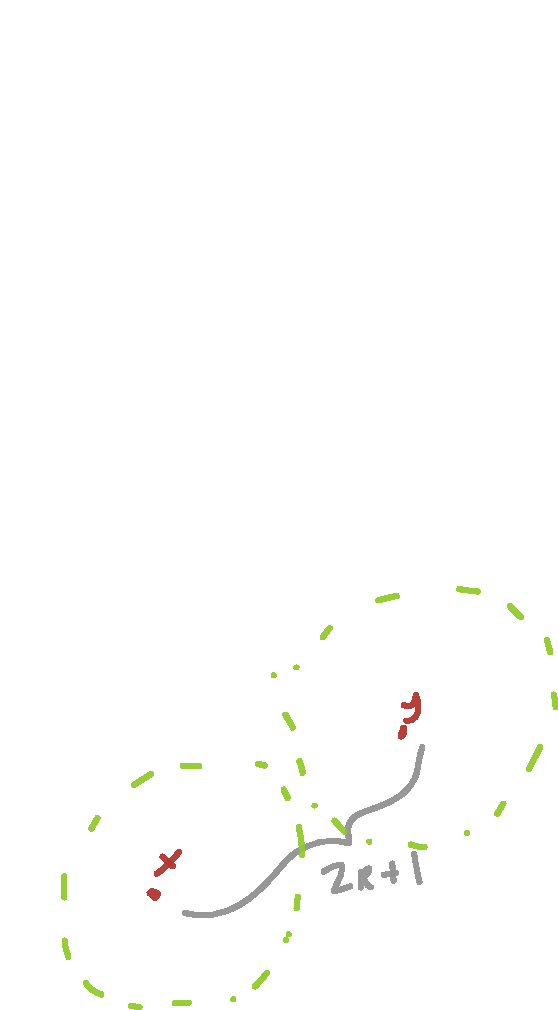
\includegraphics[scale=0.5]{img/img2.pdf}

\subsection{Linjära koder}
$C$ är en linjärkod om
$$ x+y\in C, \all x,y\in C $$

\subsubsection{Exempel}
$$(1011)^T+(0110)^T=(1101)^T$$ är kodord
$ 0=x+x\in C$
$d(x,0) = $ antal ettor i $x$
$d(C) =$ minsta antalet ettor som förekommer i ett kodord $\neq 0$.

\subsection{Konstruktion av kod med 4 meddelanden (fem bitar)}
Välj alla binära tal $x=x_1 x_2 x_3 x_4 x_5$ så att
$$
H\begin{cases}
x_1+x_2+x_4+x_5=0\\
x_1+x_3+x_5=0\\
x_1+x_3+x_4=0
\end{cases}
$$
$C =$ nollrummet till matrisen H \uline{kontrollmatris}

\subsection{Eliminera (binärt)}
$$
\begin{cases}
x_1=x_3+x_5\\
x_2=x_3+x_5\\
x_4=_4
\end{cases}
$$

\begin{tabular}{ l l | l l l | l l l l l }
$x_3$ & $x_5$ & $x_1$ & $x_2$ & $x_4$ & $x_1$ & $x_2$ & $x_3$ & $x_4$ & $x_5$ \\\hline
0 & 0 & 0 & 0 & 0 & 0 & 0 & 0 & 0 & 0\\
0 & 1 & 1 & 1 & 1 & 1 & 1 & 0 & 1 & 1\\
1 & 0 & 1 & 1 & 0 & 1 & 1 & 1 & 0 & 0\\
1 & 1 & 0 & 0 & 1 & 0 & 0 & 1 & 1 & 1\\
\end{tabular}
$$d(C)=3=2\times 1+1$$
2 fel upptäcks\\
1 fel kan rättas

\subsection{}
$$ x\to y, Hy=0 $$
$$ Hy\neq 0 $$
Om fel $y=x+e$,
där e är felvekorn.
$$x=01101\to 01111=y=x+e=01101+00010$$
$$ Hy=H(x+e)=Hx+He=He $$
$$ H(0 0 1 0)^T=(1 0 1)^T\eq
\pmat{1&1&0&1&1\\
1 &0&1&0&1\\
1&0&1&1&0}
(0 0 0 1 0)^T =(1 0 1)^T
$$
\subsection{Exempel}
Normalform för H
$$
\pmat{
1&0&0& 1&1&0\\
0&1&0 &1&0&1\\
0&0&1 &0&1&1
}
\left(
x_1 x_2 x_3 x_4 x_5 x_5 x_6
\right)^T =
\left(
0 0 0
\right)^T =
$$
$$ C=\{ 000000, 01101, 101010, 110011, 110100, 101101, 011110, 000111 \} $$
$$ d(C)=3 $$
Upptäck 2 fel.
Rätta 1 fel.

\subsection{Sats}
$C_1, C_2$ linjära koder.
Då är
$$ C=\{(x,x+y);x\in C, y\in C_2 \} $$
en linjär kod. Vidare $d(C)=$ minsta av $2\times d(C_1)$ och $d(C_2)$

\subsection{Exempel}
$$ C_1 = \{00,01,10,11\}, C_2=\{00,11\} $$
$$ d(C_1) = 1, d(C_2)=2 $$
$$ C =\{0000, 0011, 0100, 0111, 1000, 1011, 1100, 1111\} $$
$$ d(C) = 2$$

\subsection{Exempel}
Mariner 9 (1971).
$ C_1 =\{ $ alla $ x=x_1x_2x_3x_4 $så att$ x_1+x_2+x_3+x_4=0 \} $
$$ C_1 =\{ 0000, 1111 \} $$
$$ d(C_1) =2, d(C_2)=4$$
Satsen ger $C_1'$ med $d(C_1')=4$\\
Med $C_2' = \{00000000, 11111111\}, d(C_2')=8$\\
Satsen ger $C_1''$ med $d(C_2'')=8, C_2''=\{0000000000000000,1111111111111111\}$ ger $C$ med $d(C)=16\ge 15=2\times 7+1$

\subsection{}
$$ 7\times 9 = 63 = 5\times 11+8 \equiv 8 $$
Bilda koder $x_1 x_2\dots x_1, 11^{10}$
$$
\begin{cases}
  x_1+x_2+x_3+\dots+x_{10}=0\ (mod\ 11)\\
  x_1+2x_2+3x_3+\dots+10x_{10}=0\ (mod\ 11)\\
\end{cases}
$$
ger 82644629 koder utan 10.
rättar ett fel.

\end{document}
